%%%%%%%%%%%%%%%%%%%%%%%%%%%%%%%%%%%%%%%%%%%%%%%%%%%%%%%%%%%%%%%%%%
%%%%%%%%%%%%%%%%%%%%%%%%%%%%%%%%%%%%%%%%%%%%%%%%%%%%%%%%%%%%%%%%%%
%Packages
\documentclass[10pt, a4paper]{article}
\usepackage[top=3cm, bottom=4cm, left=3.5cm, right=3.5cm]{geometry}
\usepackage{amsmath,amsthm,amsfonts,amssymb,amscd, fancyhdr, color, comment, graphicx, environ}
\usepackage{float}
\usepackage{mathrsfs}
\usepackage[math-style=ISO]{unicode-math}
\setmathfont{TeX Gyre Termes Math}
\usepackage{lastpage}
\usepackage[dvipsnames]{xcolor}
\usepackage[framemethod=TikZ]{mdframed}
\usepackage{enumerate}
\usepackage[shortlabels]{enumitem}
\usepackage{fancyhdr}
\usepackage{indentfirst}
\usepackage{listings}
\usepackage{sectsty}
\usepackage{thmtools}
\usepackage{shadethm}
\usepackage{hyperref}
\usepackage{setspace}
\usepackage[linguistics]{forest}
\hypersetup{
    colorlinks=true,
    linkcolor=blue,
    filecolor=magenta,      
    urlcolor=blue,
}
%%%%%%%%%%%%%%%%%%%%%%%%%%%%%%%%%%%%%%%%%%%%%%%%%%%%%%%%%%%%%%%%%%
%%%%%%%%%%%%%%%%%%%%%%%%%%%%%%%%%%%%%%%%%%%%%%%%%%%%%%%%%%%%%%%%%%
%Environment setup
\mdfsetup{skipabove=\topskip,skipbelow=\topskip}
\newrobustcmd\ExampleText{%
An \textit{inhomogeneous linear} differential equation has the form
\begin{align}
L[v ] = f,
\end{align}
where $L$ is a linear differential operator, $v$ is the dependent
variable, and $f$ is a given non−zero function of the independent
variables alone.
}
\mdfdefinestyle{theoremstyle}{%
linecolor=black,linewidth=1pt,%
frametitlerule=true,%
frametitlebackgroundcolor=gray!20,
innertopmargin=\topskip,
}
\mdtheorem[style=theoremstyle]{Problem}{Problem}
\newenvironment{Solution}{\textbf{Solution.}}

\definecolor{codegreen}{rgb}{0,0.6,0}
\definecolor{codegray}{rgb}{0.5,0.5,0.5}
\definecolor{codepurple}{rgb}{0.58,0,0.82}
\definecolor{backcolour}{rgb}{0.95,0.95,0.92}

\lstdefinestyle{mystyle}{
    backgroundcolor=\color{backcolour},   
    commentstyle=\color{codegreen},
    keywordstyle=\color{magenta},
    numberstyle=\tiny\color{codegray},
    stringstyle=\color{codepurple},
    basicstyle=\ttfamily\footnotesize,
    breakatwhitespace=false,         
    breaklines=true,                 
    captionpos=b,                    
    keepspaces=true,                 
    numbers=left,                    
    numbersep=5pt,                  
    showspaces=false,                
    showstringspaces=false,
    showtabs=false,                  
    tabsize=2
}

\lstset{style=mystyle}
%%%%%%%%%%%%%%%%%%%%%%%%%%%%%%%%%%%%%%%%%%%%%%%%%%%%%%%%%%%%%%%%%%
%%%%%%%%%%%%%%%%%%%%%%%%%%%%%%%%%%%%%%%%%%%%%%%%%%%%%%%%%%%%%%%%%%
%Fill in the appropriate information below
\newcommand{\norm}[1]{\left\lVert#1\right\rVert}     
\newcommand\course{EES405}                            % <-- course name   
\newcommand\hwnumber{Lab Assignment-01}                                 % <-- homework number
\newcommand\Information{(Shiv Shankar Singh)}% <-- personal information
\newcommand\Roll{(MS18006)}
%%%%%%%%%%%%%%%%%%%%%%%%%%%%%%%%%%%%%%%%%%%%%%%%%%%%%%%%%%%%%%%%%%
%%%%%%%%%%%%%%%%%%%%%%%%%%%%%%%%%%%%%%%%%%%%%%%%%%%%%%%%%%%%%%%%%%
%Page setup
\pagestyle{fancy}
\headheight 35pt
\lhead{\today}
\rhead{
\includegraphics[width=2.5cm]{iisermlogo.jpg}}
\lfoot{}
\pagenumbering{arabic}
\cfoot{\small\thepage}
\rfoot{}
\headsep 1.2em
\renewcommand{\baselinestretch}{1.25}
%%%%%%%%%%%%%%%%%%%%%%%%%%%%%%%%%%%%%%%%%%%%%%%%%%%%%%%%%%%%%%%%%%
%%%%%%%%%%%%%%%%%%%%%%%%%%%%%%%%%%%%%%%%%%%%%%%%%%%%%%%%%%%%%%%%%%
%Add new commands here
\renewcommand{\labelenumi}{\alph{enumi})}
\newcommand{\Z}{\mathbb Z}
\newcommand{\R}{\mathbb R}
\newcommand{\Q}{\mathbb Q}
\newcommand{\NN}{\mathbb N}
\newcommand{\PP}{\mathbb P}
\DeclareMathOperator{\Mod}{Mod} 
\renewcommand\lstlistingname{Algorithm}
\renewcommand\lstlistlistingname{Algorithms}
\def\lstlistingautorefname{Alg.}
\newtheorem*{theorem}{Theorem}
\newtheorem*{lemma}{Lemma}
\newtheorem{case}{Case}
\newcommand{\assign}{:=}
\newcommand{\infixiff}{\text{ iff }}
\newcommand{\nobracket}{}
\newcommand{\backassign}{=:}
\newcommand{\tmmathbf}[1]{\ensuremath{\boldsymbol{#1}}}
\newcommand{\tmop}[1]{\ensuremath{\operatorname{#1}}}
\newcommand{\tmtextbf}[1]{\text{{\bfseries{#1}}}}
\newcommand{\tmtextit}[1]{\text{{\itshape{#1}}}}

\newenvironment{itemizedot}{\begin{itemize} \renewcommand{\labelitemi}{$\bullet$}\renewcommand{\labelitemii}{$\bullet$}\renewcommand{\labelitemiii}{$\bullet$}\renewcommand{\labelitemiv}{$\bullet$}}{\end{itemize}}
\catcode`\<=\active \def<{
\fontencoding{T1}\selectfont\symbol{60}\fontencoding{\encodingdefault}}
\catcode`\>=\active \def>{
\fontencoding{T1}\selectfont\symbol{62}\fontencoding{\encodingdefault}}
\catcode`\<=\active \def<{
\fontencoding{T1}\selectfont\symbol{60}\fontencoding{\encodingdefault}}

%%%%%%%%%%%%%%%%%%%%%%%%%%%%%%%%%%%%%%%%%%%%%%%%%%%%%%%%%%%%%%%%%%
%%%%%%%%%%%%%%%%%%%%%%%%%%%%%%%%%%%%%%%%%%%%%%%%%%%%%%%%%%%%%%%%%%
%Begin now!



\begin{document}

\begin{titlepage}
    \begin{center}
        \vspace*{3cm}
            
        \Huge
        \textbf{Climate data analysis and Visualization (EES405)}
            
        \vspace{1cm}
        \huge
        \hwnumber
            
        \vspace{1.5cm}
        \Large
            
        \textbf{\Information}                      % <-- author
        
            
        \vfill
        
        \course
            
        \vspace{1cm}
            
        
\includegraphics[width=0.4\textwidth]{iisermlogo.jpg}
        \\
        
        \Large
        
        \today
            
    \end{center}
\end{titlepage}

%%%%%%%%%%%%%%%%%%%%%%%%%%%%%%%%%%%%%%%%%%%%%%%%%%%%%%%%%%%%%%%%%%
%%%%%%%%%%%%%%%%%%%%%%%%%%%%%%%%%%%%%%%%%%%%%%%%%%%%%%%%%%%%%%%%%%
%Start the assignment now
%%%%%%%%%%%%%%%%%%%%%%%%%%%%%%%%%%%%%%%%%%%%%%%%%%%%%%%%%%%%%%%%%%
%New problem
\newpage
Lab Assignment-01
\subsubsection*{Plot vertical thermal structure of the atmosphere using NCEP/NCAR long-term mean data for summer (JJAS mean), winter (DJF mean) and annual (mean of Jan-Dec) using Python.}

\begin{Problem}
\begin{enumerate}
    \item Vertical Thermal structure of the Globe (0-360E $\&$  90S – 90N)
    \item Vertical Thermal structure of the Tropics (0-360E $\&$ 30S – 30N)
    \item Vertical Thermal structure of the North Pole (0-360E $\&$ 70N – 90N)
    \item Vertical Thermal structure over India (60-110E $\&$ 6N – 35N)
\end{enumerate}
\end{Problem}

\begin{Solution}

% Example of a lemma.
% \begin{lemma}
%     This is a lemma.
% \end{lemma}

% Example of a proof.
% \begin{proof}
%     Write your proof here.
% \end{proof}

% Example of including a picture.
% \begin{center}
%     
\includegraphics[width = 4cm]{iisermlogo.jpg}
% \end{center}

% Example of referring to a piece of code.
% \lstinputlisting[language = python]{Program Solution.py}

% Example of a table.
% \begin{equation*}\begin{tabular}{ c c c }
%                 & Mean          & SD \\ 
%      Fall 2077  & 7.046512      & 1.714552 \\  
%      Fall 1977  & 9.102941      & 1.568919
% \end{tabular}\end{equation*}

% Overall, this is a quite basic template for assignments, and above are only some basic features. I included enough packages and set a few environments. You may modify them or add features to fit your personal preference. Enjoy using it!

I plotted the vertical thermal structure of different regions (Globally, Tropics (-30,30), North Pole (70,90) and India) across three different seasons (Summer (JJAS), winter (DJF), and annual mean). \\
I followed the following protocol/steps in generating all the above plots. \\

\begin{enumerate}
    \item \textbf{Step:1} Load the data in an array format with xarray library
    \item \textbf{Step:2} Take mean of the data along latitude, longitude and time axis 
    \item \textbf{Step:3} Generate plot with data.mean along x-axis and pressure levels along y-axis
    \end{enumerate}
For python source code to execute the above task, see Appendix.\\
\subsection*{Plots generated}
% Vertical thermal structure of different regions across seasons
\subsubsection{Vertical Thermal structure over India (60-110E $\&$ 6N – 35N)}

\begin{figure}[b]
    \centering
    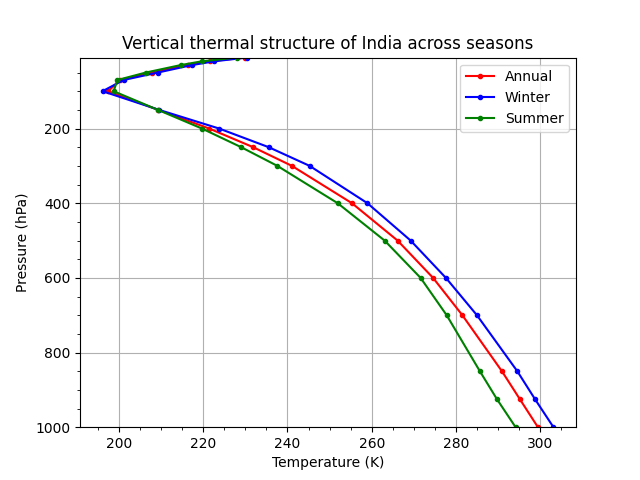
\includegraphics[width=0.33\textwidth]{india_seasons.png}
    \caption{Vertical Thermal structure over India (60-110E $\&$ 6N – 35N)}
    \label{fig:my_label}
\end{figure}
Here, we can see that there are almost no changes in the vertical thermal structure going up into the atmosphere, as India lies in the tropical region. The convection setup helps in the regulation of the temperature profile across seasons.

\newpage
Lab Assignment-01
\subsubsection{Vertical thermal structure of Tropics (0-360 $\&$ 30S-30N)}
As expected, since the tropics receive the same amount of sunlight throughout the year and there are no significant changes in the solar flux received across the seasons, hence the vertical temperature profile is almost the same across the seasons.
\begin{figure}[h]
    \centering
    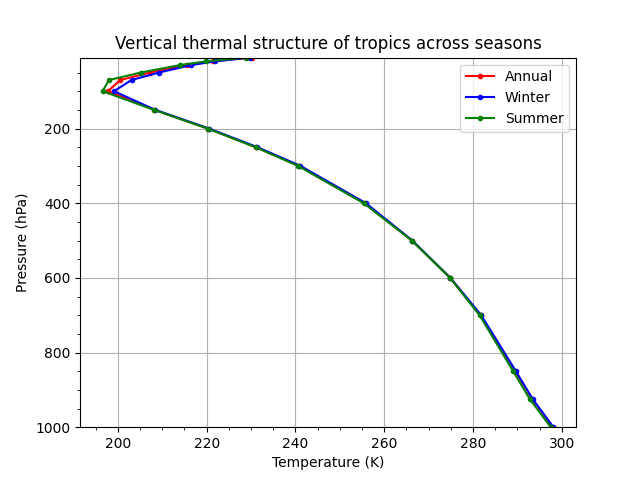
\includegraphics[width=0.5\textwidth]{tropics_seasons.png}
    \caption{Vertical thermal structure of Tropics (0-360 $\&$ 30S-30N)}
    \label{fig:my_label}
\end{figure}

\subsubsection{Vertical thermal structure of North Pole (0-360 $\&$ 70N-90N)}

Since, the amount of sunlight received by the north pole varies drastically across seasons, the same can be inferred from vertical thermal structure over north pole, where we can see that the profiles of different seasons(summer and winter) are quite spread apart from each other.

\begin{figure}[h]
    \centering
    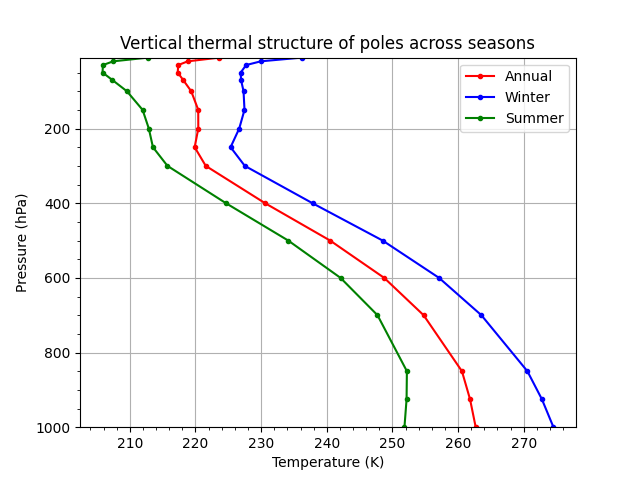
\includegraphics[width=0.5\textwidth]{poles_seasons.png}
    \caption{Vertical thermal structure of North Pole (0-360 $\&$ 70N-90N)}
    \label{fig:my_label}
\end{figure}

\newpage
Lab Assignment-01
\subsubsection{Vertical thermal structure of globe}
The vertical thermal profile averaged over the whole of the globe doesn't seem to vary much as the annual budget of sunlight received doesn't change across the seasons (summer in the northern hemisphere is compensated by winter in the southern hemisphere and vice versa) as it is averaged over the entire globe.
\begin{figure}[h]
    \centering
    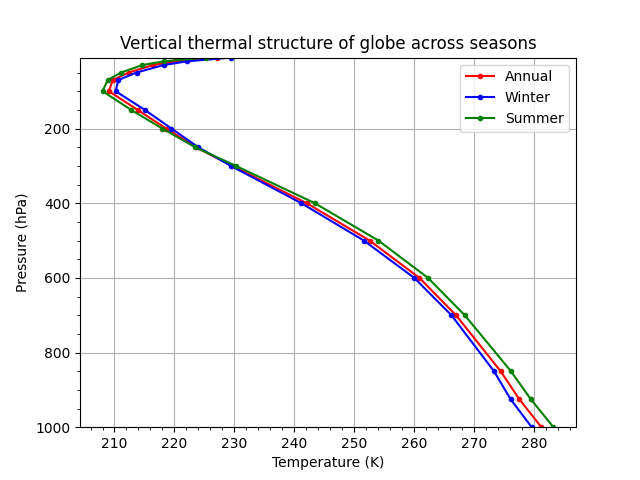
\includegraphics[width=0.45\textwidth]{global_seasons.png}
    \caption{Vertical thermal structure of globe}
    \label{fig:my_label}
\end{figure}

\subsubsection{Vertical thermal structure of different regions in summer}
As discussed above, we can see the vertical thermal structure of the poles is very different as compared to the tropics. Certain visible characteristics are:
\begin{itemize}
    \item Based on the definition of the troposphere as discussed in the class, we can see that troposphere height is more near the tropics and equator and less near the north pole.
    \item The tropopause temperature is also different for the poles and tropics/equatorial region. \\ North pole has tropopause temperature, which is almost 20-25 deg C lower as compared to the tropics/equatorial regions.
\end{itemize}
 \begin{figure}[h]
     \centering
     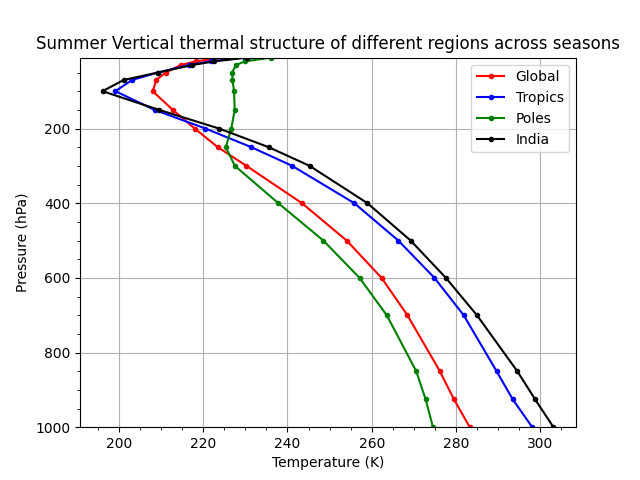
\includegraphics[width=0.45\textwidth]{summer_regions.png}
     \caption{Vertical thermal structure of different regions in summer}
     \label{fig:my_label}
\end{figure}

\newpage
Lab Assignment-01
\subsubsection{Vertical thermal structure of different regions in winter}
 Similar to what we see in the summer season, but the difference between the tropopause temperature of the tropics/equatorial region is less as compared to the north pole (almost 10-15 deg C).
 \begin{figure}[h]
     \centering
     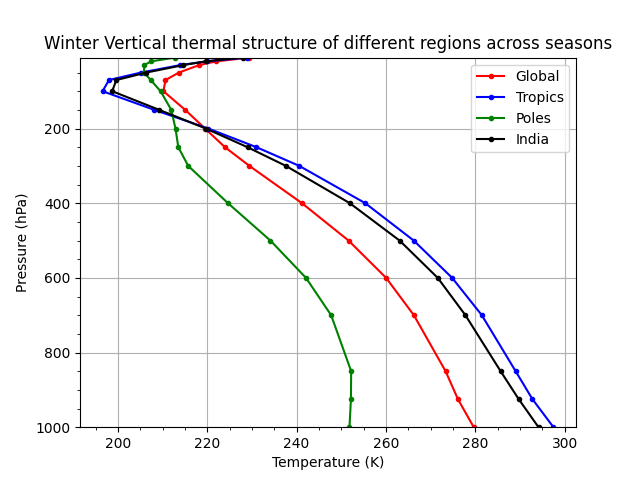
\includegraphics[width=0.5\textwidth]{winter_regions.png}
     \caption{Vertical thermal structure of different regions in winter}
     \label{fig:my_label}
 \end{figure}


\end{Solution}

\vspace{1cm}
\hline
\vspace{1cm}


\subsubsection*{Spatial distribution of Diurnal temperature range for pre-summer season (M, A
M months) using Climate Research Unit data. Follow the steps:}
\begin{Problem}
\begin{enumerate}
    \item Select MAM months from CRU Tmin data for the period 1980-2020.
    \item Select MAM months from CRU Tmax data for the period 1980-2020.
    \item Average for entire time period for both Tmax and Tmin files
    \item Find difference between Tmax and Tmin
    \item You will get Diurnal temperature range
\end{enumerate}
\end{Problem}

\begin{Solution}
    Did the following steps to get the diurnal temperature range from 1981-2020\\
    \begin{itemize}
        \item Merged the decade files into one file, which contains the tmn and tmx data from 1981 to 2020 (replace tmn for tmx for tmx data) \\
        \textcolor{blue}{cdo -r -f nc merge 1981.1991.tmn.nc 1991.2000.tmn.nc 2001.2010.tmn.nc 2011.2020.tmn.nc 1981.2020.tmn.nc}
    \end{itemize}
    \newpage
    Lab Assignment-01
    \vspace{1cm}
    \begin{itemize}
        \item Select the MAM (March, April and May) months from 1981.2020.tmx/n.nc file \\
        \textcolor{blue}{cdo -r -f nc selmon,3,4,5 1981.2020.tmn/x.nc 1981.2020.MAM.nc}

        \item These data files were imported into python and further analysis was carried out
        \begin{enumerate}
            \item Taking mean along time dimension \\
            \textcolor{blue}{tmn/xMean = tmx/nMAM.mean(dim='Time')}
            \item Difference of tmxMean and tmnMean to calculate diurnal temperature range \\
            \textcolor{blue}{tDTR = tmxMean - tmnMean}
        \end{enumerate}
        
    \end{itemize}

    \subsection{Diurnal temperature range of entire globe for MAM months over 1981-2020}

    \begin{figure}[h]
        \centering
        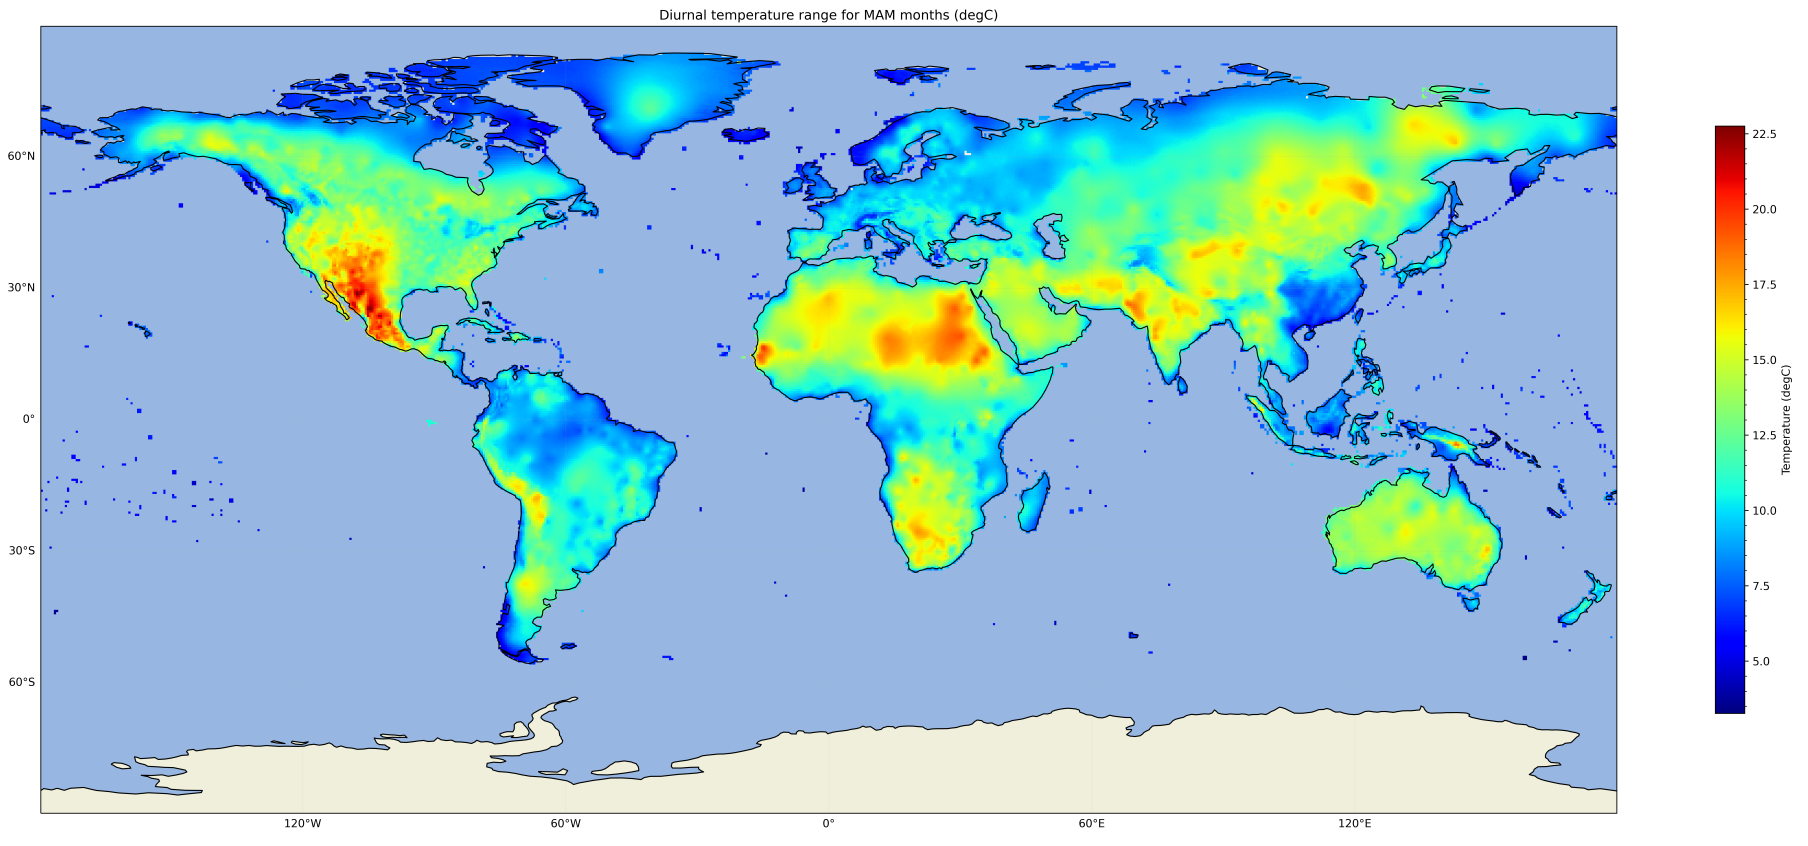
\includegraphics[width=0.8\textwidth]{Screenshot from 2023-02-11 01-10-57.png}
        \caption{Diurnal temperature range 1981-2020 for MAM months}
        \label{fig:my_label}
    \end{figure}
\end{Solution}

Here, we can see that desert regions or relatively drier regions have higher DTR as expected due to extreme temperature changes in day and night. \\

We also know that high DTR is often associated with dry and arid climates, while low DTR is associated with more humid or marine climates. Therefore, the high DTR in the Sahara and Thar regions indicates a dry climate, while the low DTR in the coastal regions suggests a more moderate or humid climate.

\newpage
Lab Assignment-01

\subsection*{Compute and plot standard deviation of JJAS precipitation anomalies over India using CRU Data for the period 1980-2015? Reference (1960-1990)}
\begin{Problem}
    Compute and plot standard deviation of JJAS precipitation anomalies over India using CRU Data for the period 1980-2015? Reference (1960-1990)
\end{Problem}

\begin{Solution}
    Did the following steps to get the JJAS precipitation anomalies over India.
    \begin{itemize}
        \item Extract the reference data and 1980-2105 dataset from CRU dataset main file. \\
        \textcolor{blue}{cdo -r -f nc selyear,1960/1990 cru.pre.nc 1960.1990.pre.nc} \\
        \textcolor{blue}{cdo -r -f nc selyear,1980/2015 cru.pre.nc 1980.2015.pre.nc}

        \item Extract JJAS (June, July, August and September) months from both the datasets \\
        \textcolor{blue}{cdo -r -f nc selmon.6,7,8,9 1960.1990.pre.nc 1960.1990.JJAS.pre.nc}\\
        \textcolor{blue}{cdo -r -f nc selmon.6,7,8,9 1980.2015.pre.nc 1980.2015.JJAS.pre.nc} 

        \item Estimate the climatology from the reference data (1960-1990) \\
        \textcolor{blue}{cdo -r -f nc timmean 1960.1990.pre.nc mean.nc}

        \item Estimate anomalies defined as $\text{Anomaly } = (X_i - \bar{X}) $, where $\bar{X}$ is the climatology \\
        \textcolor{blue}{cdo -r -f nc sub 1980.2015.JJAS.pre.nc anomaly.nc}

        \item Compute the standard deviation of anomalies calculated above \\
        \textcolor{blue}{cdo -r -f nc timstd anomaly.nc anomaly.std.nc}
        
        \end{itemize}

        \begin{figure}[h]
            \centering
            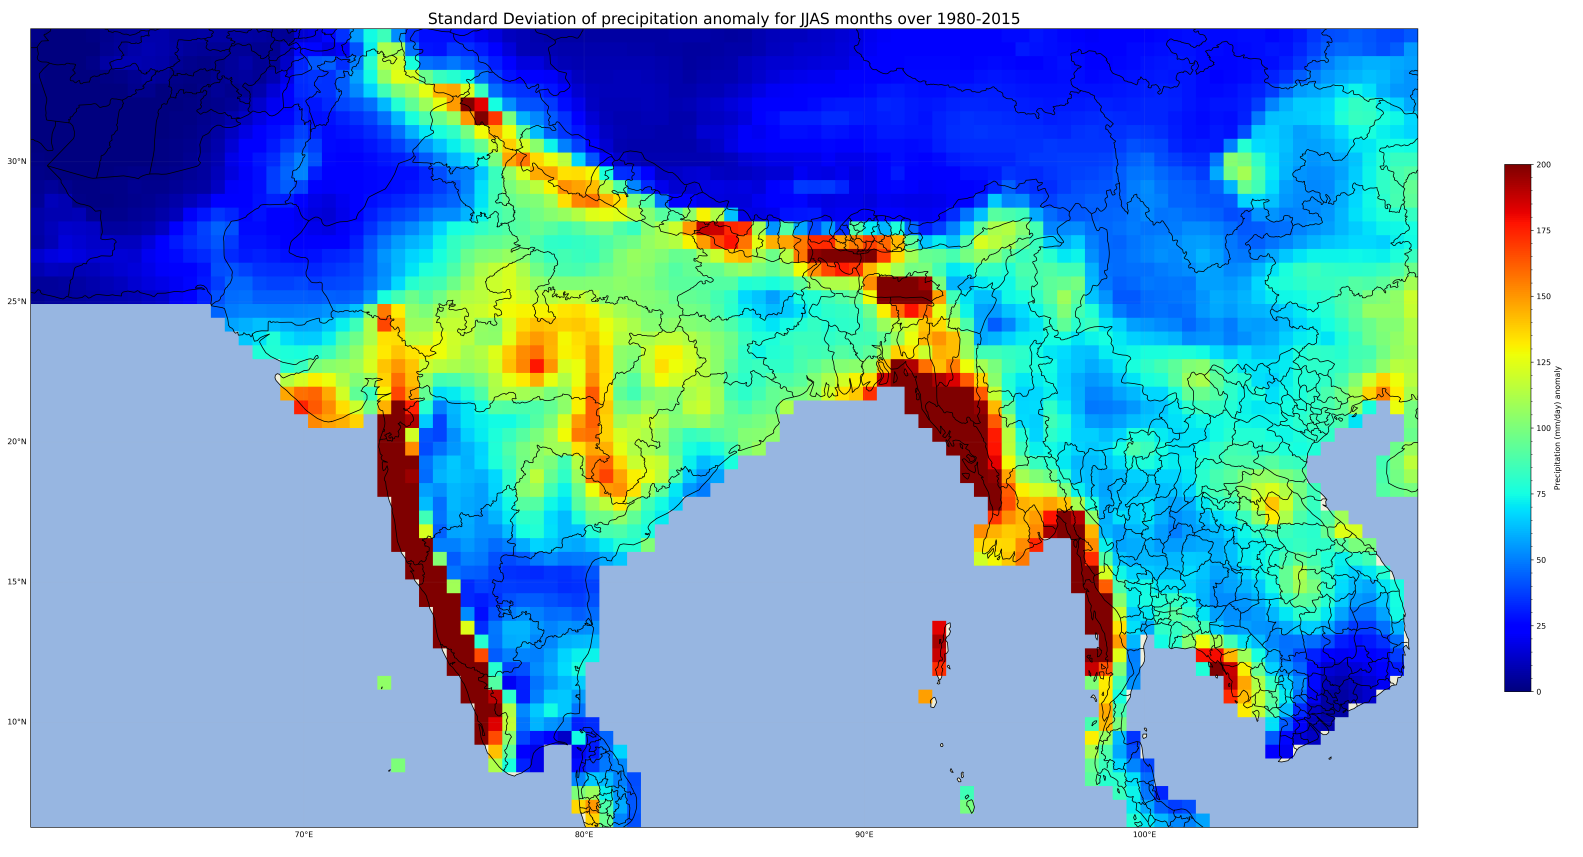
\includegraphics[width=0.65\textwidth]{india-spatial.png}
            \caption{Standard Deviation of precipitation anomaly for JJAS months over 1980-2015.png}
            \label{fig:my_label}
        \end{figure}
We can see that coastal regions have high precipitation anomalies as compared to inland regions and desert and arid regions as precipitation is more likely to be unpredictable in high precipitation regions and hence more standard deviation of precipitation anomalies (more spread of the anomalies data).        
\end{Solution}

\newpage
Lab Assignment-01
\subsection*{Find time series of correlation between precipitation and mean temperature from CRU data.}
\begin{Problem}
    \begin{enumerate}
        \item Extract MAMJJASON period for both the variable from 1990-2010
        \item Estimate Climatology
        \item Correlates all grid points of the two variables. (Time series)
    \end{enumerate}
\end{Problem}

\begin{Solution}
    Did the following steps to get the correlation between temperature and precipitation for MAMJJASON months
    \begin{itemize}
        \item Extract the dataset for the period of 1990-2010 from main CRU datafile\\
        \textcolor{blue}{cdo -r -f nc selyear,1990/2010 cru.tmp.nc 1990.2010.tmp.nc}\\
        \textcolor{blue}{cdo -r -f nc selyear,1990/2010 cru.pre.nc 1990.2010.pre.nc}

        \item Extract MAMJJASON (Mar., Apr., June, July, Aug., Sept. Oct. Nov.) from the dataset \\
        \textcolor{blue}{cdo -r -f nc selmon,3/11 1990.2010.tmp.nc 1990.2010.tmp.MAMJJASON.nc} \\
        \textcolor{blue}{cdo -r -f nc selmon,3/11 1990.2010.pre.nc 1990.2010.pre.MAMJJASON.nc}

        \item Estimate climatology \\
        \textcolor{blue}{cdo -r -f nc timmean 1990.2010.tmp.MAMJJASON.nc mean.tmp.nc} \\
        \textcolor{blue}{cdo -r -f nc timmean 1990.2010.pre.MAMJJASON.nc mean.pre.nc}

        \item Correlating the grid points (Time series) \\
        \textcolor{blue}{cdo -r -f nc fldcor mean.tmp.nc mean.pre.nc tmp.pre.fldcor.nc}

        
    \end{itemize}
    \begin{figure}[h]
        \centering
        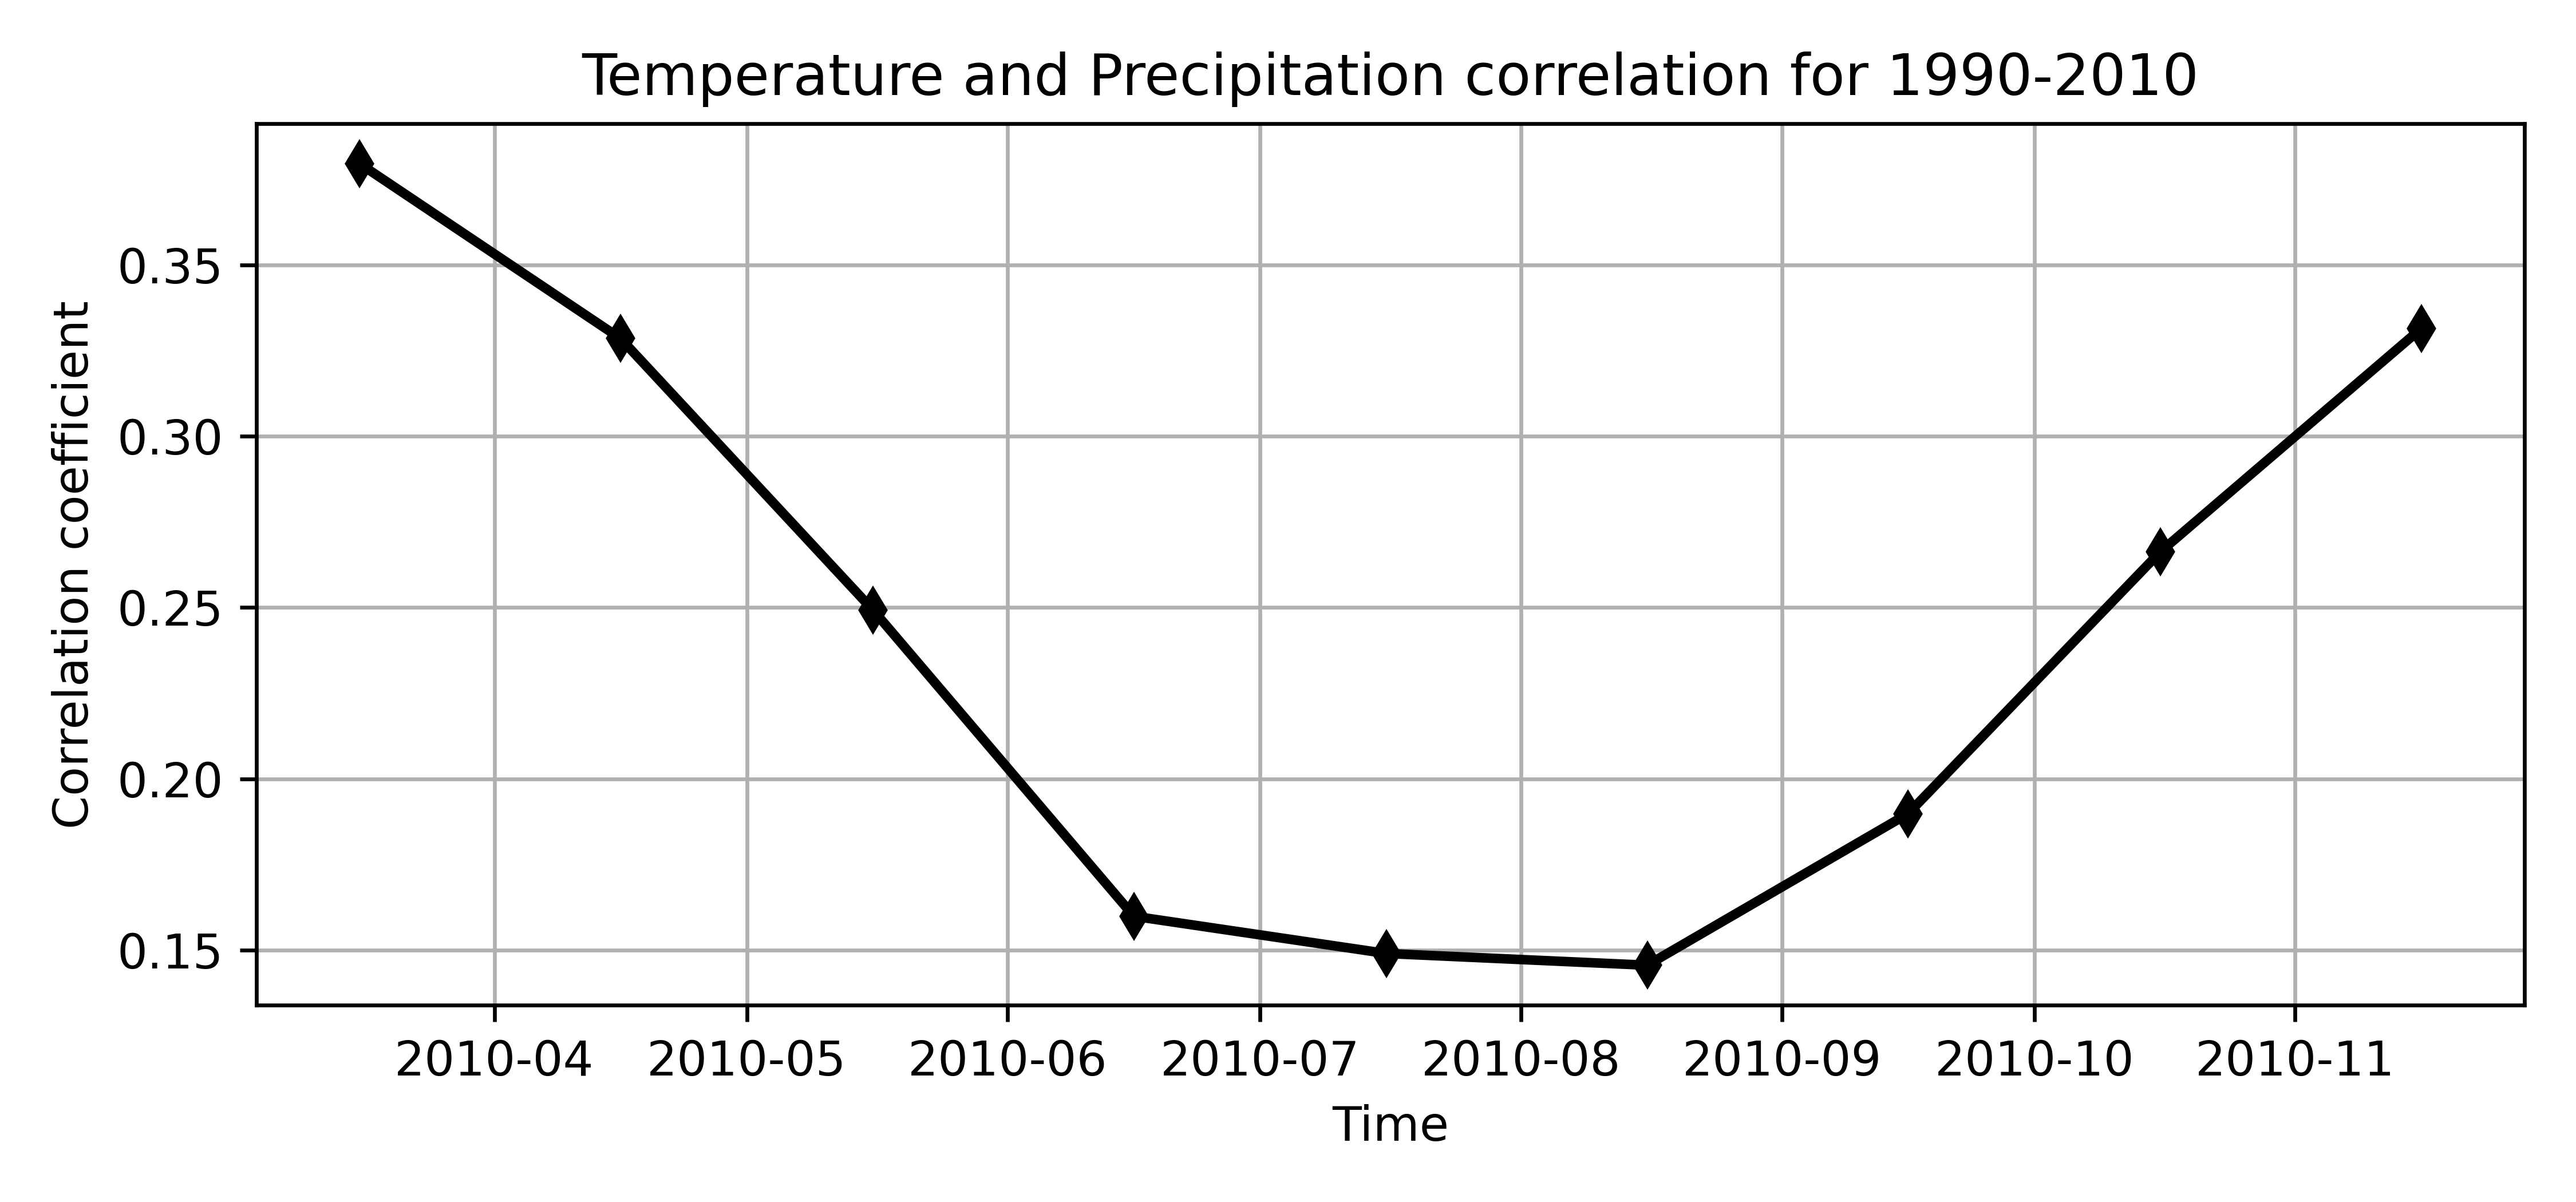
\includegraphics[width=0.75\textwidth]{Temperature and Precipitation correlation for 1990-2010.png}
        \caption{Temperature and Precipitation correlation for 1990-2010}
        \label{fig:my_label}
    \end{figure}

    Here, we can see that there exists higher positive correlation between temperature and precipitation during non-monsoon months, and higher temperature drives the oncoming of precipitation, but as soon as the monsoon season starts, the correlation between the two
    \newpage
    Lab Assignment-01
    \vspace{1cm}
    
    variables weaken, and we see that there is very less correlation between temperature and precipitation during monsoon months. We should acknowledge that temperature is not the only driving factor of precipitation during monsoon season, and there are multiple factors affecting precipitation during these months; hence we can expect a weaker correlation between temperature and precipitation during monsoon seasons.
\end{Solution}

\subsection*{Spatial map of correlation between precipitation and mean temperature from CRU data.}

\begin{Problem}
    \begin{enumerate}
        \item Extract JJA period for both the variable from 1990-2010
        \item Estimate Climatology (ymonmean)
        \item Correlation at each grid point for all times of the two variables
    \end{enumerate}
\end{Problem}

\begin{Solution}
    Followed the same steps as above, except for the last part of the spatial correlation between temperature and precipitation.
    \begin{itemize}
        % \item Extract the dataset for the period of 1990-2010 from main CRU datafile\\
        % \textcolor{blue}{cdo -r -f nc selyear,1990/2010 cru.tmp.nc 1990.2010.tmp.nc}\\
        % \textcolor{blue}{cdo -r -f nc selyear,1990/2010 cru.pre.nc 1990.2010.pre.nc}

        % \item Extract JJA (June, July, August) from the dataset \\
        % \textcolor{blue}{cdo -r -f nc selmon,6/8 1990.2010.tmp.nc 1990.2010.tmp.JJA.nc} \\
        % \textcolor{blue}{cdo -r -f nc selmon,6/8 1990.2010.pre.nc 1990.2010.pre.JJA.nc}

        % \item Estimate climatology \\
        % \textcolor{blue}{cdo -r -f nc timmean 1990.2010.tmp.JJA.nc mean.tmp.nc} \\
        % \textcolor{blue}{cdo -r -f nc timmean 1990.2010.pre.JJA.nc mean.pre.nc}

        \item Correlating the grid points (Spatial map) \\
        \textcolor{blue}{cdo -r -f nc timcor mean.tmp.nc mean.pre.nc tmp.pre.timcor.nc}

        
    \end{itemize}

    \begin{figure}[htb]
        \centering
        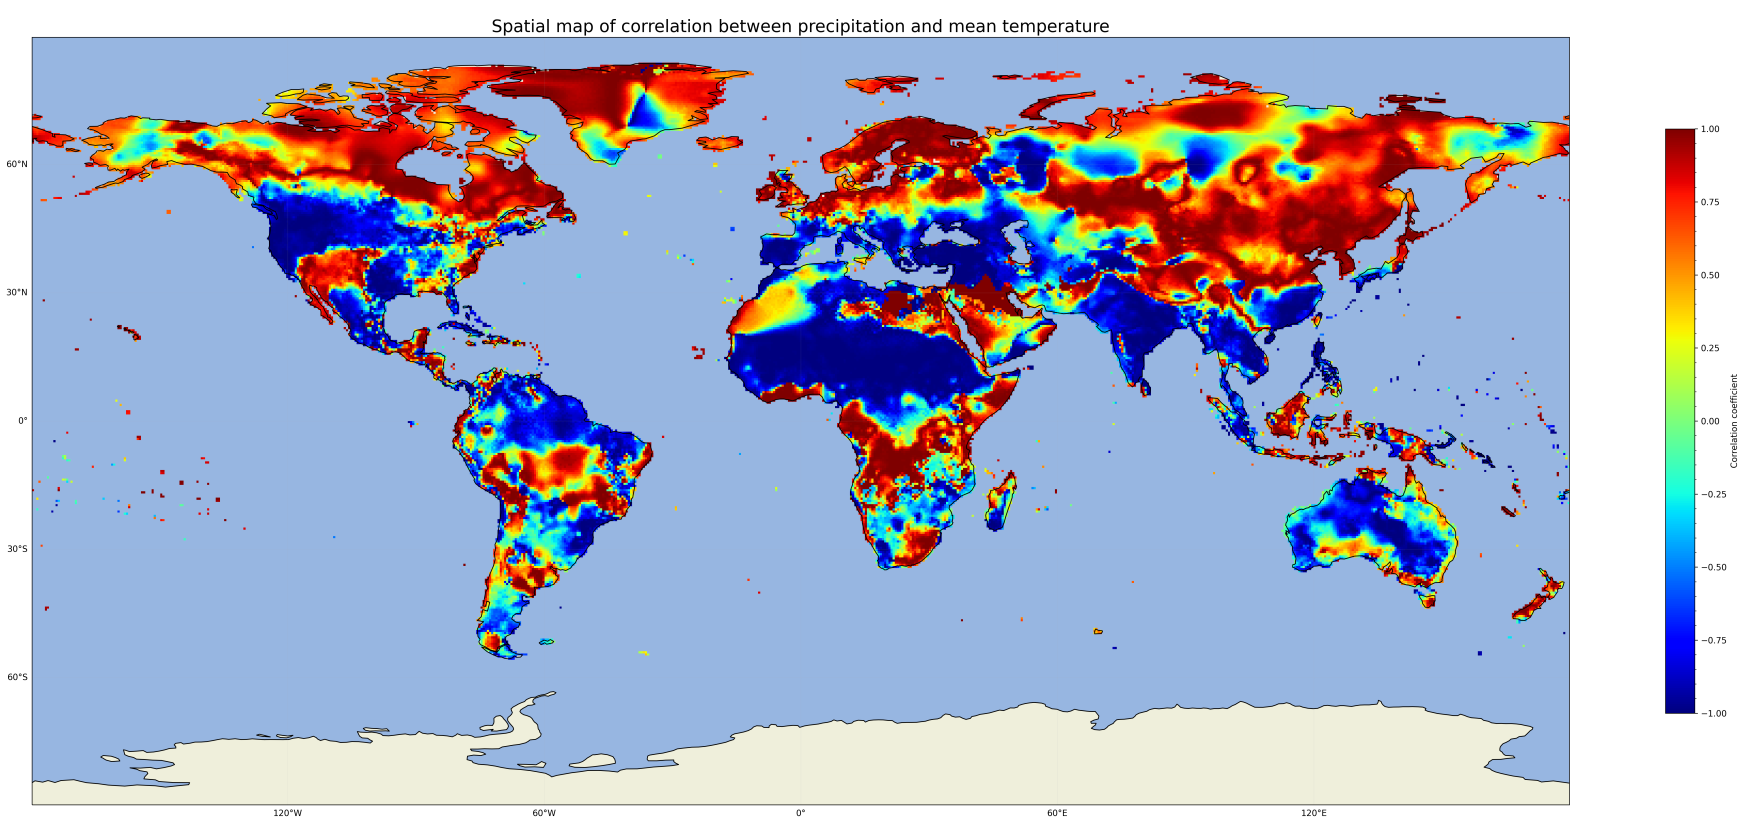
\includegraphics[width=0.85\textwidth]{spatial-correlation-tmp-pre.png}
        \caption{Spatial map of correlation between precipitation and mean temperature}
        \label{fig:my_label}
    \end{figure}

    From the plot, we can see a positive correlation in the equatorial regions where higher temperature drives the precipitation, and higher tropics or desert regions have a negative correlation coefficient. 
    
\end{Solution}

\newpage
Lab Assignment-01
\vspace{0.25cm}
\subsection*{Spatial map of correlation between precipitation from CRU data and outgoing longwave radiation from NOAA dataset.}

\begin{Problem}
    \begin{enumerate}
        % \item Use CRU precipitation data and NOAA OLR Data.
        \item Remap them (CRU => NOAA)
        \item Plot spatial correlation between them during JJA season
    \end{enumerate}
\end{Problem}

\begin{Solution}
    Did the following steps to get the spatial correlation of precipitation data from CRU and OLR data from NOAA
    \begin{itemize}
        \item Used the climatology data of precipitation from earlier problem \\
        \textcolor{blue}{cru.pre.mean.nc}
        \item Estimate climatology of OLR data from NOAA \\
        \textcolor{blue}{cdo -r -f nc timmean olr.noaa.nc olr.noaa.mean.nc} 
        \item Regrid the NOAA dataset(2.5deg) to match the resolution of CRU dataset (0.5deg)
        \begin{itemize}
            \item Getting the grid description from cru dataset and storing it into a text file \\
            \textcolor{blue}{cdo -r -f nc griddes cru.pre.mean.nc > gridrefdata}
            \item Using the grid description file to regrid the NOAA dataset\\
            \textcolor{blue}{cdo -r -f nc remapbil,gridrefdata olr.noaa.mean.nc remap.olr.mean.nc}
        \end{itemize}

        \item Estimate spatial correlation between precipitation and OLR \\
        \textcolor{blue}{cdo timcor remap.olr.mean.nc cru.pre.mean.nc olr.pre.nc}
    \end{itemize}

\begin{figure}[h]
    \centering
    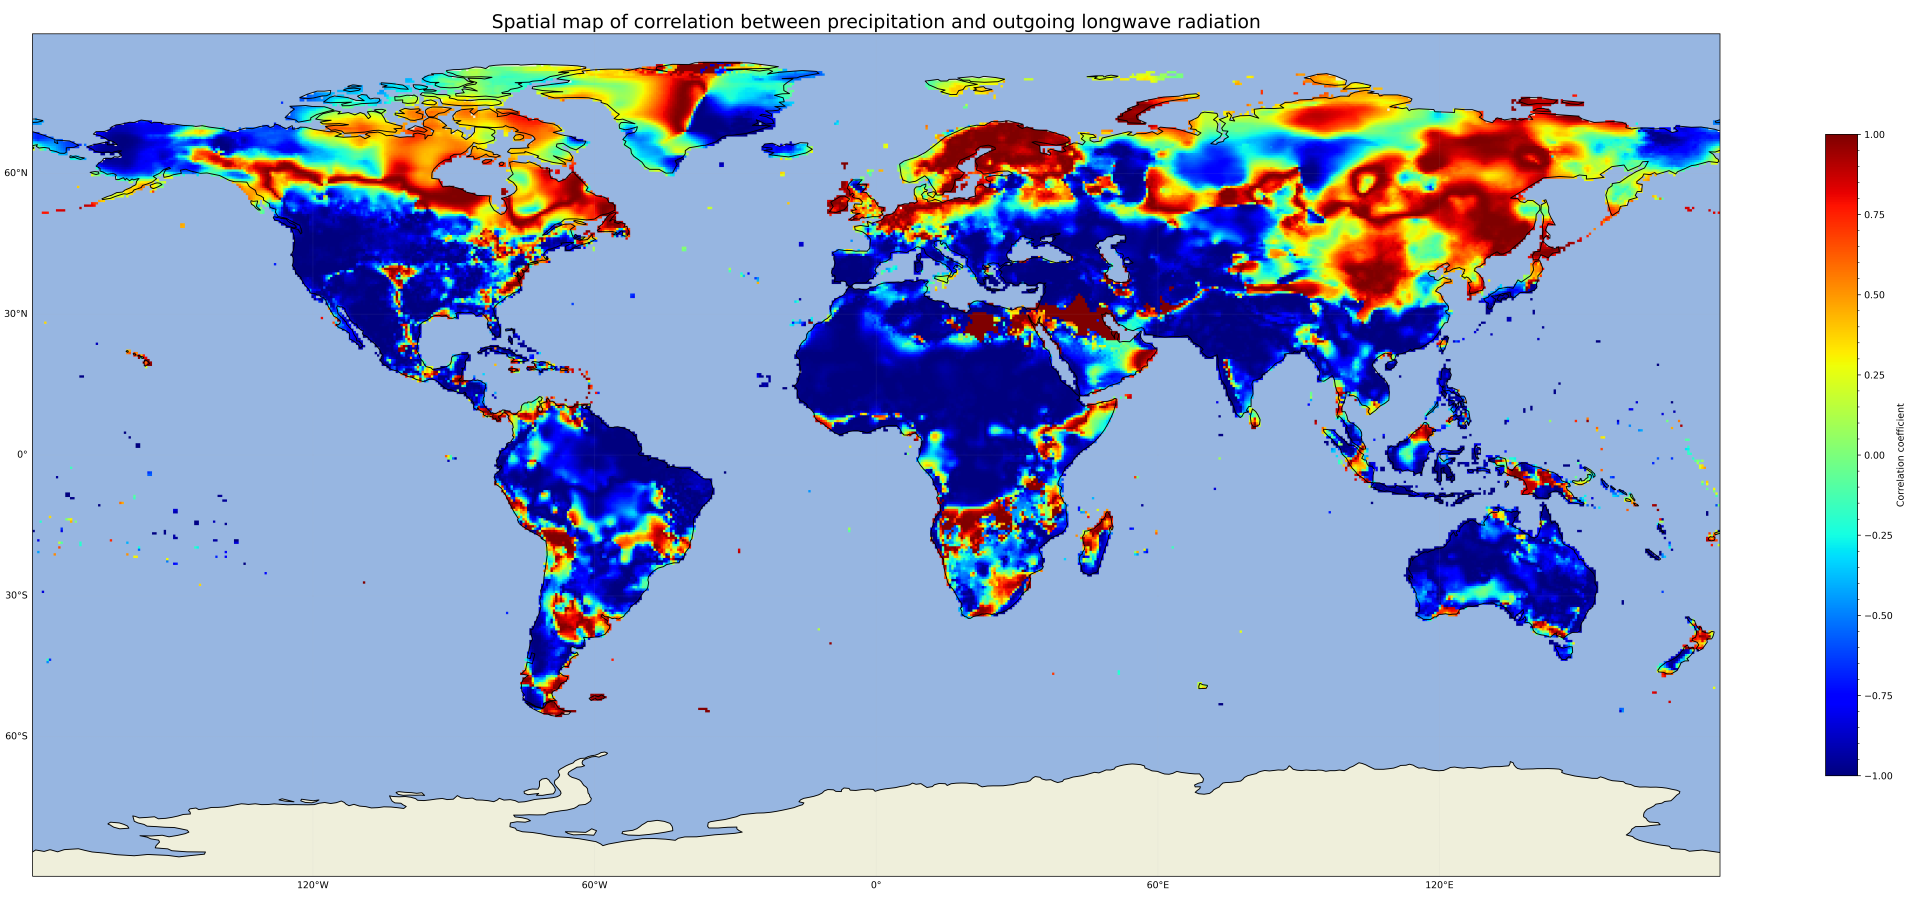
\includegraphics[width=0.85\textwidth]{spatial-correlation-pre-olr.png}
    \caption{Spatial map of correlation between precipitation and outgoing longwave radiation}
    \label{fig:my_label}
\end{figure}

In regions with high moisture content, such as tropical rainforests or coastal areas, there is typically a negative correlation between OLR and precipitation. This is because high 

\newpage
Lab Assignment-01 \\

\vspace{1cm}
moisture content leads to cloud formation and increased absorption of outgoing longwave radiation, which can result in lower OLR and increased precipitation.

However, the relationship between OLR and precipitation may be more complex in drier regions. For example, high OLR values may indicate a lack of atmospheric moisture and a lower likelihood of precipitation in some arid or semi-arid regions. In other cases, high OLR values may be associated with the presence of high-altitude clouds, which can trap longwave radiation and contribute to the warming of the atmosphere but may not necessarily result in precipitation.
    
\end{Solution}

\subsection{Year to Year Variation of (Time evolution) of area-averaged of hot season (MAM) temperatures (seasonal anomalies normalized with standard deviation) over CIR.}
\begin{Problem}
    Year to Year Variation of (Time evolution) of area-averaged of hot season (MAM) temperatures (seasonal anomalies normalized with standard deviation) over CIR.
\end{Problem}

\begin{Solution}
    


Did the following steps to get the standardized temperature anomaly over the central Indian region (CIR) for MAM months. 
\begin{itemize}
    \item Compute MAM mean for each year\\
    \textcolor{blue}{cdo selmon,3,4,5 cru.tmp.nc cru.tmp.MAM.nc} \\
    \textcolor{blue}{cdo yearmean cru.tmp.MAM.nc cru.tmp.MAM.yearmean.nc}

    \item Extract Central Indian region  \\
    \textcolor{blue}{cdo -sellonlatbox,70,88,18,28 cru.tmp.MAM.yearmean.nc cru.tmp.MAM.yearmean.CIR.nc}

    \item Compute area average of the CIR \\
    \textcolor{blue}{cdo fldmean cru.tmp.MAM.yearmean.nc cru.tmp.MAM.yearmean.fldmean.nc}

    \item Compute Climatology \\
    \textcolor{blue}{cdo timmean cru.tmp.MAM.yearmean.fldmean.nc cru.tmp.MAM.yearmean.fldmean.timmean.nc}

    \item Compute seasonal anomalies \\
    \textcolor{blue}{cdo sub cru.tmp.MAM.yearmean.fldmean.nc cru.tmp.MAM.yearmean.fldmean.timmean.nc anomaly.nc}

    \item Calculate standardized anomaly\\
    \textcolor{blue}{cdo timstd cru.tmp.MAM.yearmean.fldmean.nc cru.tmp.MAM.yearmean.fldmean.std.nc} \\

    \newpage
    Lab Assignment-01\\
    
    \vspace{1cm}
    \textcolor{blue}{cdo div anomaly.nc cru.tmp.MAM.yearmean.fldmean.std.nc anomaly.stddiv.nc}

    \item Set relative time axis \\
    \textcolor{blue}{cdo -r settaxis,1901-01-01,00:00:00,1year anomaly.stddiv.nc anomaly.stddiv.relative.nc}
\end{itemize}

\subsection*{Plots generated} 
 \subsubsection{Standardized temperature anomaly for 1901-2020} 
 \begin{figure}[h]
     \centering
     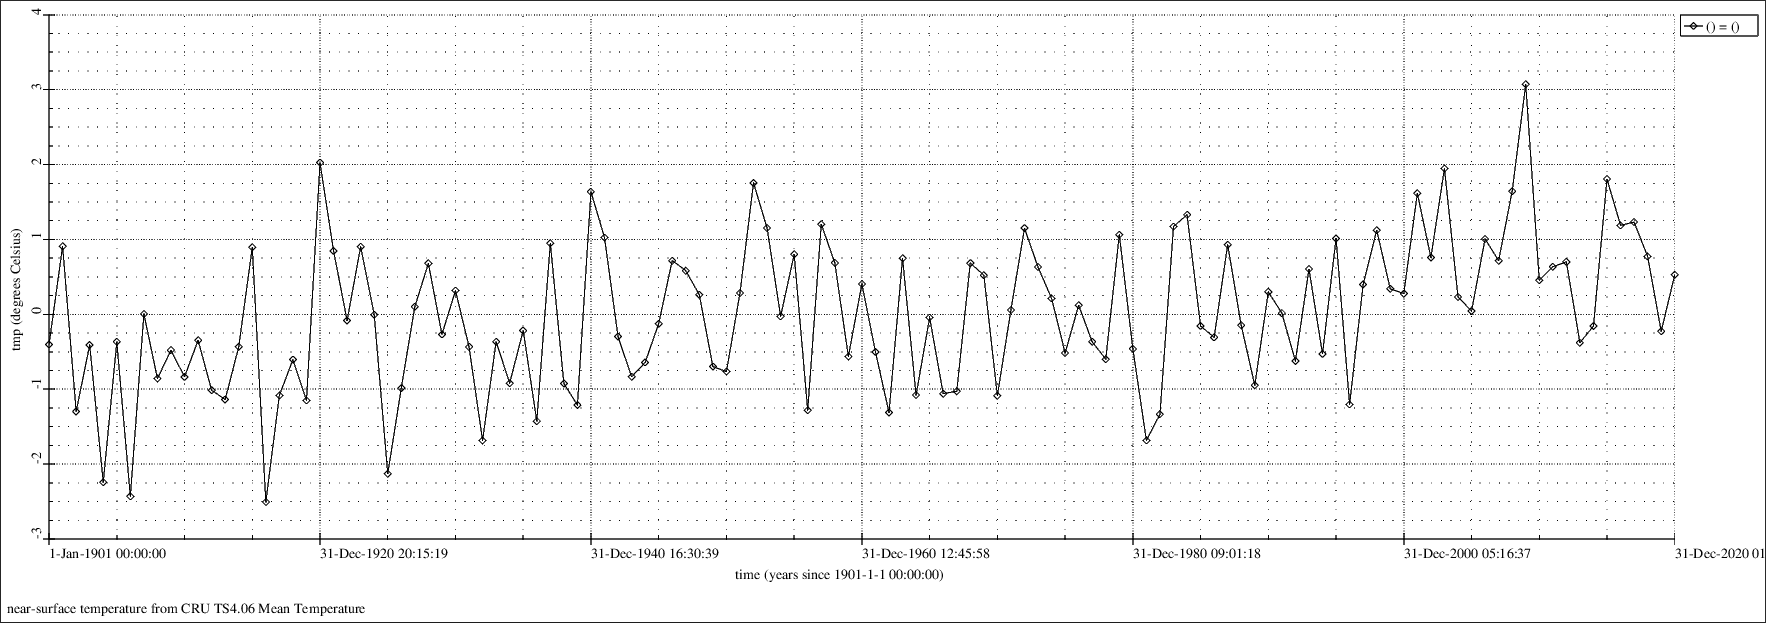
\includegraphics[width=0.85\textwidth]{stddiv-all.png}
     \caption{Standardized temperature anomaly for 1901-2020}
     \label{fig:my_label}
 \end{figure}
From the above plot, we can see an increase in the standardized temperature anomaly over the years. To better visualise the increase in the trend, let's add a trendline (linear fit to the data) and see the change
 \subsubsection{Standardized temperature anomaly for 1901-2020 with trendline} 
\begin{figure}[h]
    \centering
    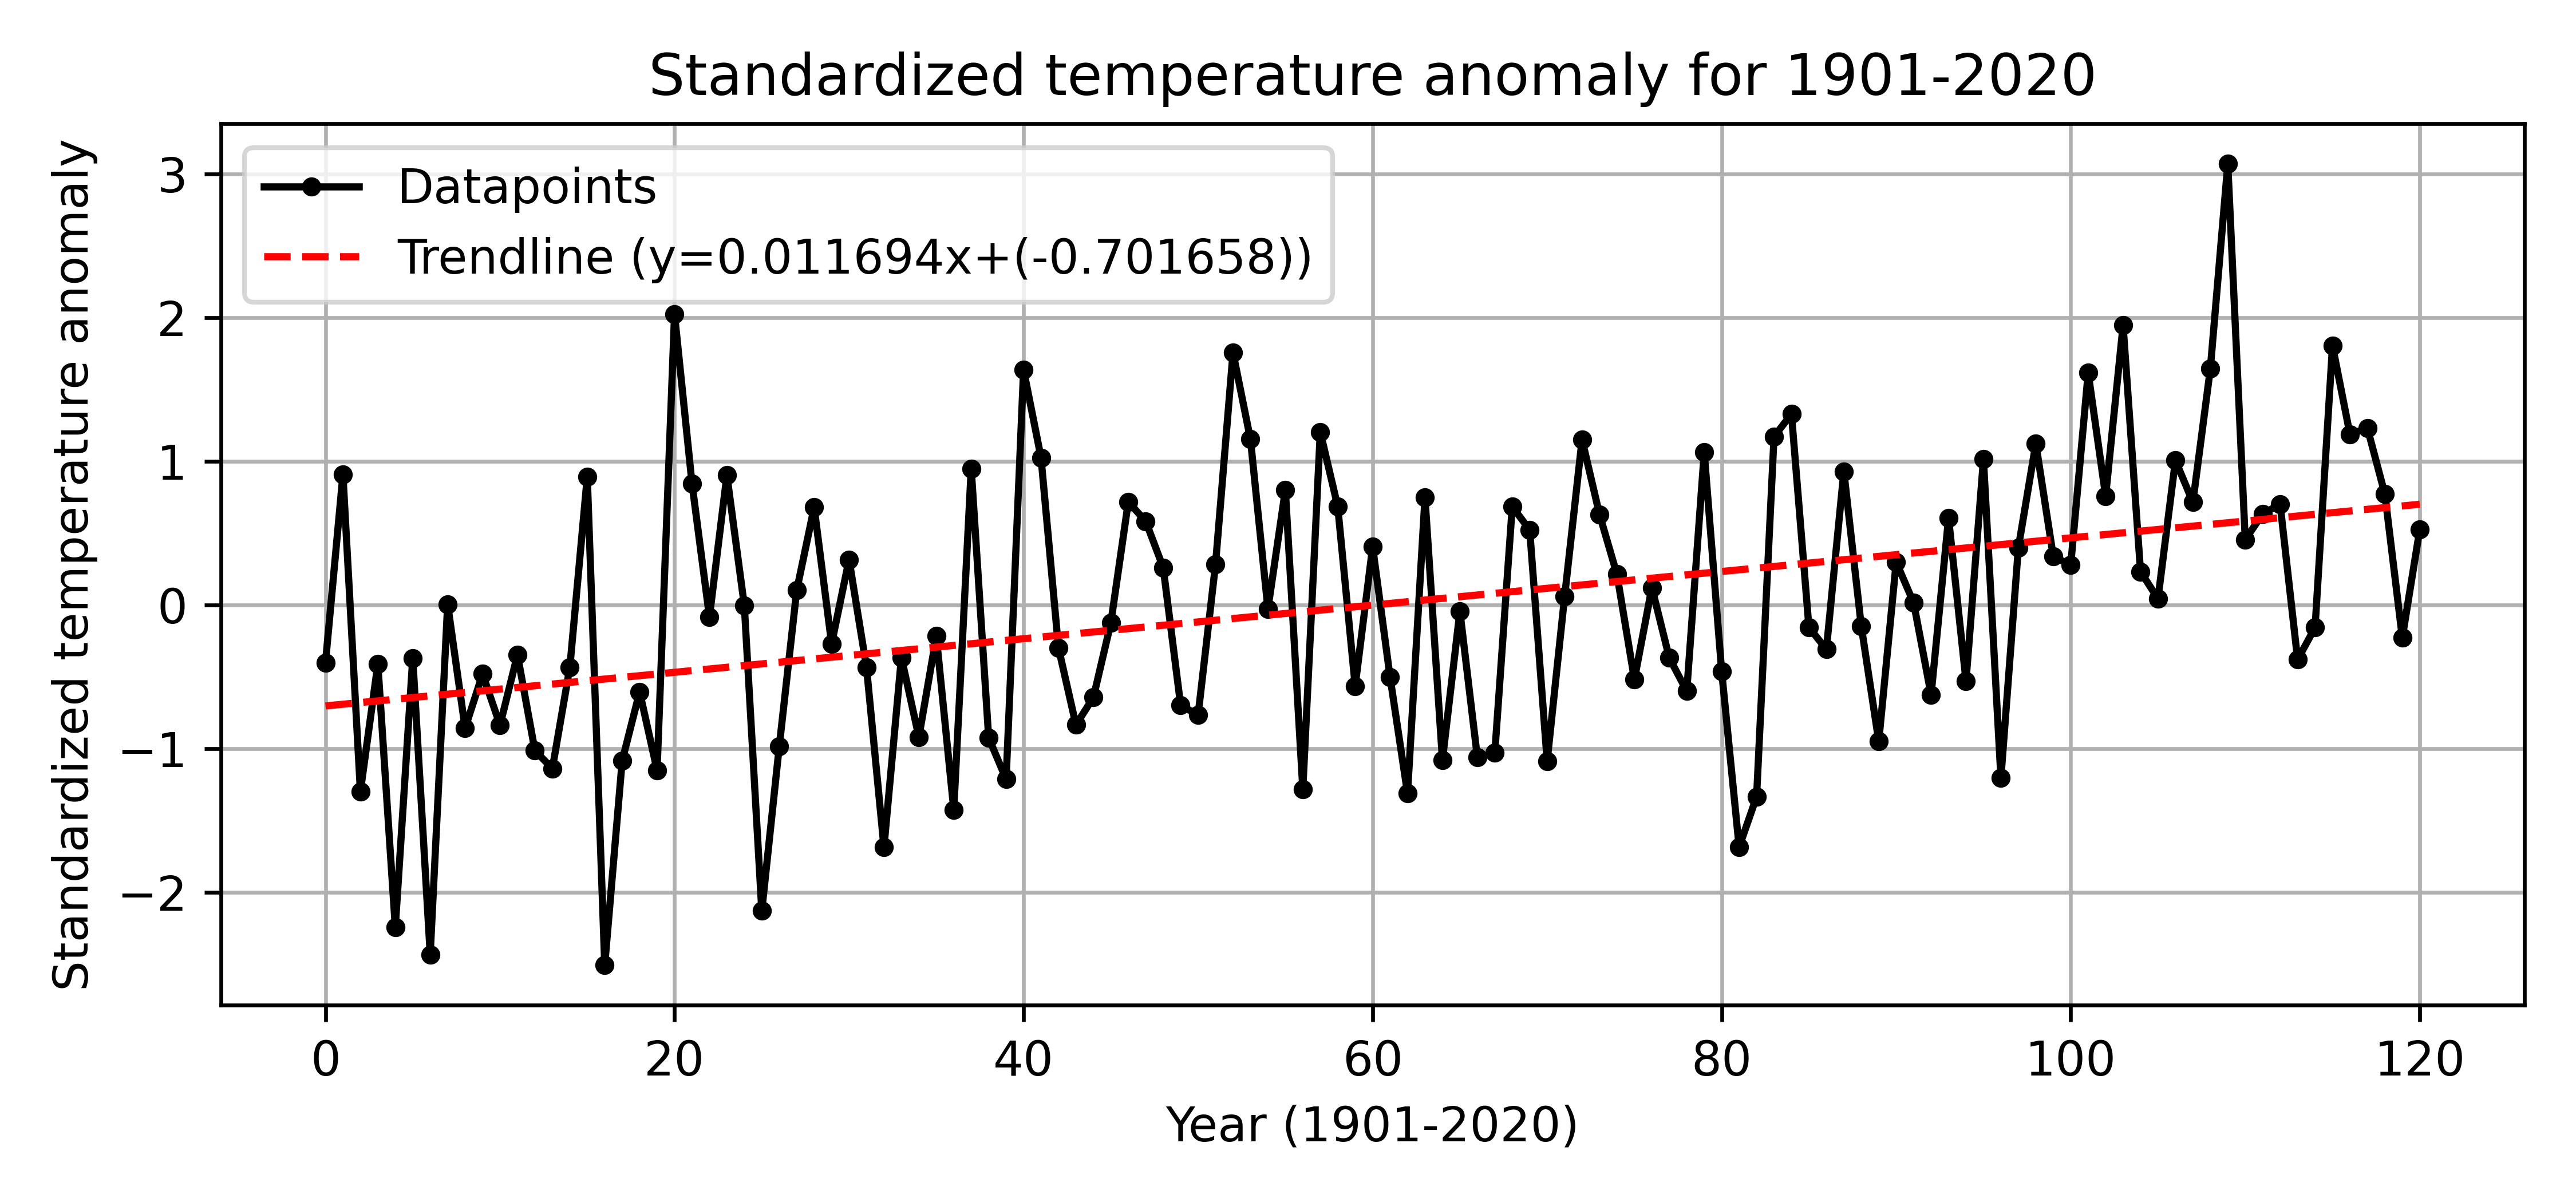
\includegraphics[width=0.85\textwidth]{Standardized temperature anomaly for 1901-2020.png}
    \caption{Standardized temperature anomaly for 1901-2020 with trendline}
    \label{fig:my_label}
\end{figure}

After adding the liner fit trend, we see an increasing trend over the years. 

\newpage
Lab Assignment-01 \\

\vspace{1cm}

I tried to reduce the time dimension from 1901-2020 to 1990-2010 to see the temperature anomaly trend in recent years and see whether the rate at which its increasing is more or less. 
 \subsubsection{Standardized temperature anomaly for 1990-2010} 
\begin{figure}[h]
    \centering
    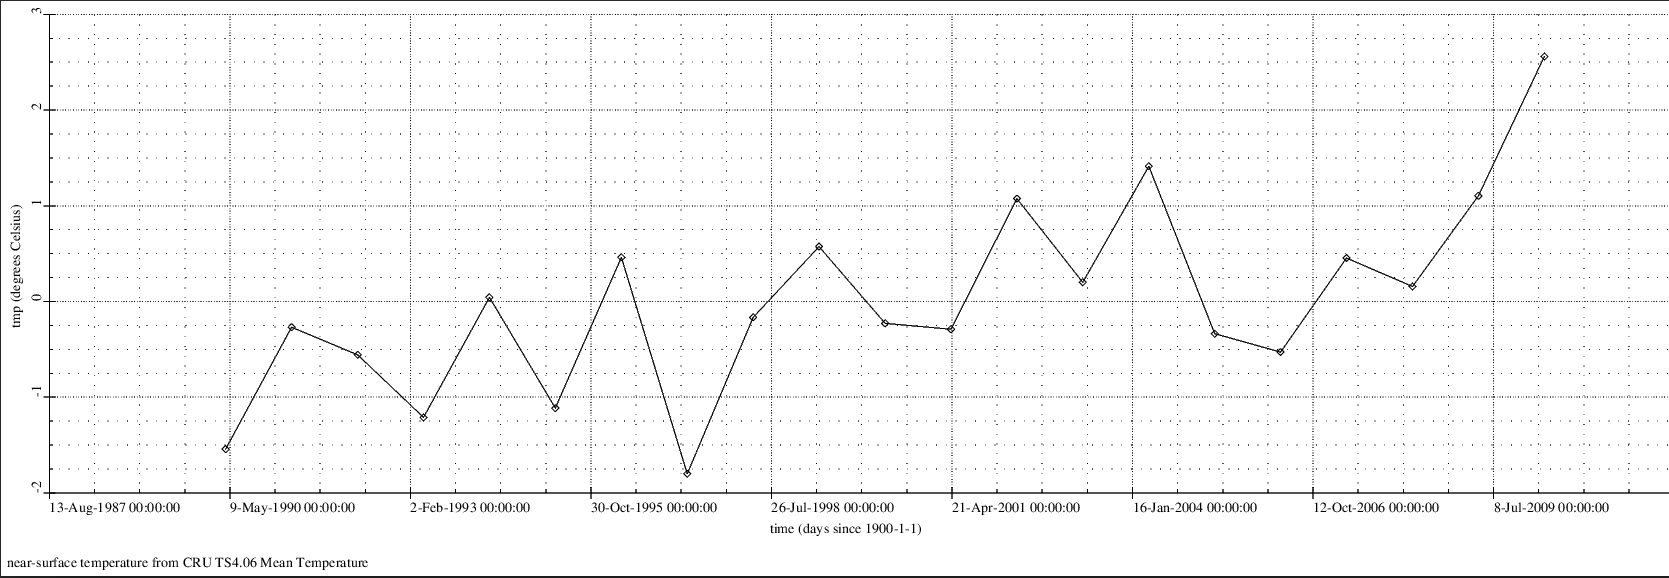
\includegraphics[width=0.85\textwidth]{stddiv-less.png}
    \caption{Standardized temperature anomaly for 1990-2010}
    \label{fig:my_label}
\end{figure}
Here, we see a more steep increase in the standardized temperature anomaly as compared to 1901-2020 plot. To better analyse the increase, let's fit the linear fit trend to datapoints and see whether the slope increases or decreases. 
 \subsubsection{Standardized temperature anomaly for 1990-2010 with trendline} 
 \begin{figure}[h]
     \centering
     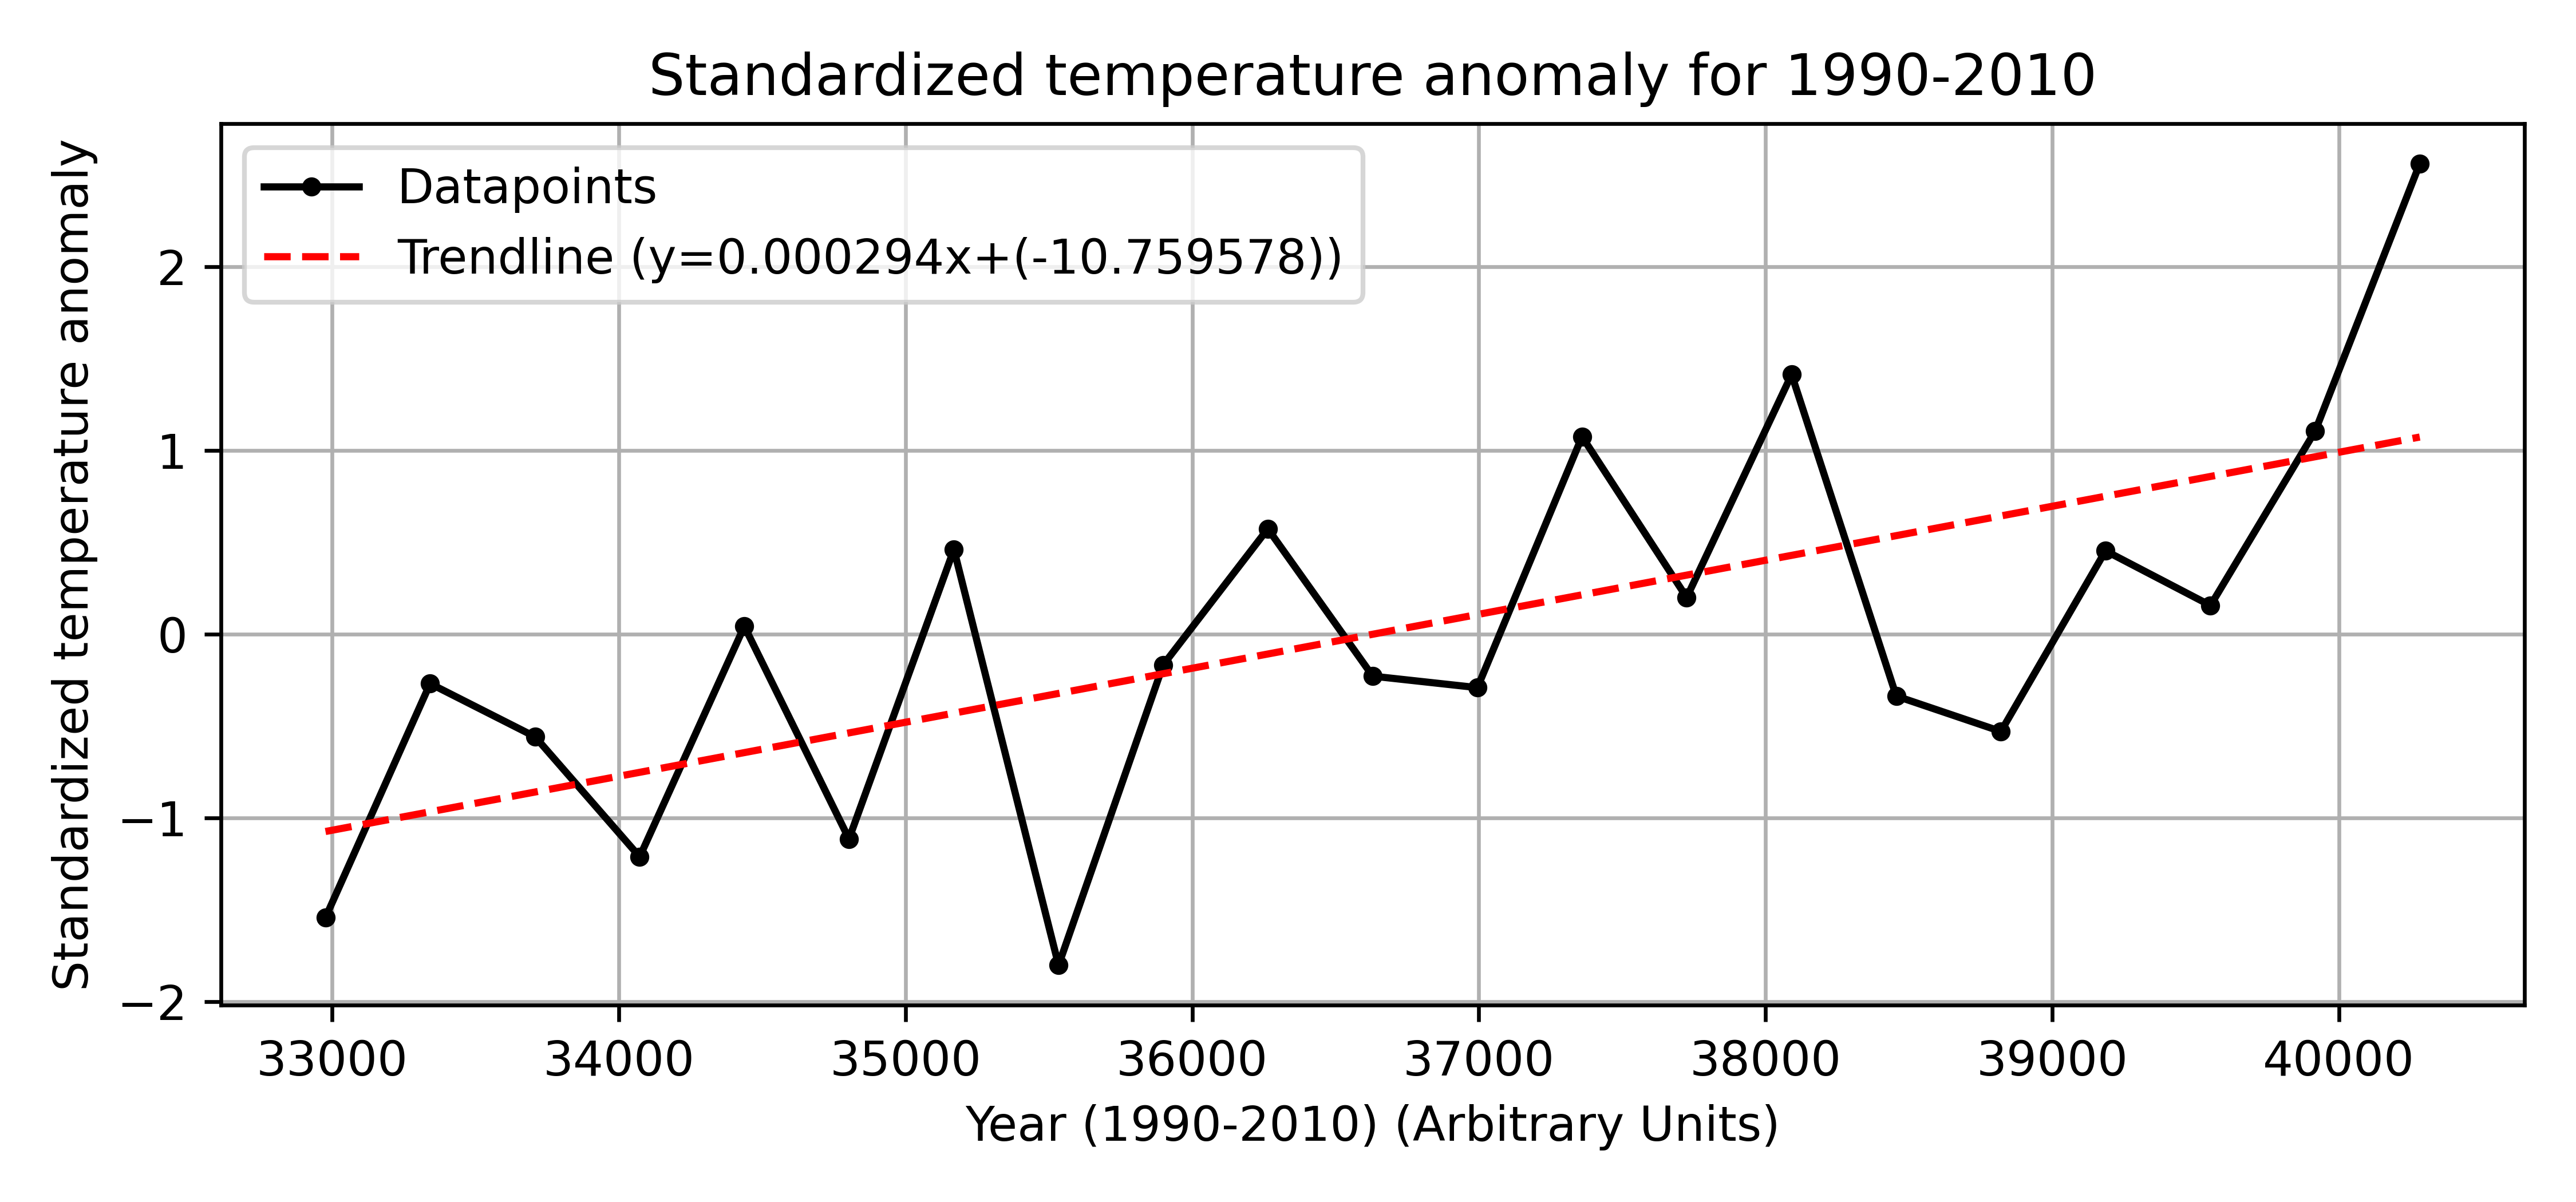
\includegraphics[width=0.85\textwidth]{Standardized temperature anomaly for 1990-2010.png}
     \caption{Standardized temperature anomaly for 1990-2010 with trendline}
     \label{fig:my_label}
 \end{figure}

From the plot, we can see that the trendline's slope is way larger compared to the 1901-2020 dataset. \textbf{Hence, we can conclude from the above plots that the temperature anomaly is not just increasing but that the rate of increase is accelerating.}

\end{Solution}



\newpage
Lab Assignment-01


\section{Appendix}

A sample code which was used to generate the vertical thermal structure plots

\lstinputlisting[language = python]{vertical_thermal_structure.py}

\newpage
Lab Assignment-01
\vspace{1cm}

Actual Python code used to generate all the vertical thermal structure plots 

\lstinputlisting[language = python]{season.py}
\vspace{1cm}
\hline
\vspace{1cm}

Python code used to generate the diurnal temperature range for MAM months from 1981-2020

\lstinputlisting[language = python]{dtr.py}

\vspace{1cm}
Python code to plot the time series and calculate the trendline from the data points plotted
\lstinputlisting[language = python]{trend.py}



%%%%%%%%%%%%%%%%%%%%%%%%%%%%%%%%%%%%%%%%%%%%%%%%%%%%%%%%%%%%%%%%%%
%Complete the assignment now
\end{document}

%%%%%%%%%%%%%%%%%%%%%%%%%%%%%%%%%%%%%%%%%%%%%%%%%%%%%%%%%%%%%%%%%%
%%%%%%%%%%%%%%%%%%%%%%%%%%%%%%%%%%%%%%%%%%%%%%%%%%%%%%%%%%%%%%%%%%
